\subsection{Hyperparameter sweep and step-invariance under fast-dLLM}
\label{sec:results-hyperparameters}

A $25$-configuration GSM8K sweep over generation length $L\in\{128, 256\}$, denoising steps $S\in\{32, 64, 128, 256\}$, and block length $B\in\{32, 64, 128, 256\}$ was run for both diffusion families before the paradigm comparison was finalized. Two findings from the sweep are relevant to the rest of the thesis.

\paragraph{Step count is a no-op for Dream under fast-dLLM.} At fixed $L=256, B=32$, Dream's pass@1 is $0.707$, $0.707$, $0.705$, $0.707$ for $S\in\{32, 64, 128, 256\}$, with wall times of $11.8$, $11.4$, $11.7$, and $12.1$ minutes. An eightfold change in nominal step count produces neither a quality nor a wall-time effect, and the same flat profile holds across every $(L, B)$ cell. LLaDA behaves oppositely: at $L=256, B=128$ its pass@1 is $0.076$, $0.397$, $0.699$, $0.710$ across the same $S$ range, and wall time scales from $3.7$ to $14.5$ minutes. Fast-dLLM therefore appears to collapse Dream's denoising into a step-count-independent operation, while LLaDA's fast-dLLM path still performs roughly $S$ sequential refinement steps. Reported Dream evaluations elsewhere in the literature that use $S=L$ are consistent with this view but spend more compute than necessary.

\paragraph{Equal-wall-time quality is comparable across diffusion families.} Dream-Base reaches pass@1$=0.707$ in $11.8$ minutes with $S=32$, while LLaDA-Base reaches pass@1$=0.699$ in $11.7$ minutes with $S=128$. The two diffusion families reach similar quality in essentially the same wall time, but trade off the $(S, B)$ knobs in opposite directions. Qwen-Base reaches pass@1$=0.730$ in $5.7$ minutes via vLLM, so the diffusion families remain slower than vLLM at equal quality on saturated math, but the wall-time gap inside the diffusion family disappears once budgets are matched.

\begin{figure}[!htbp]
\centering
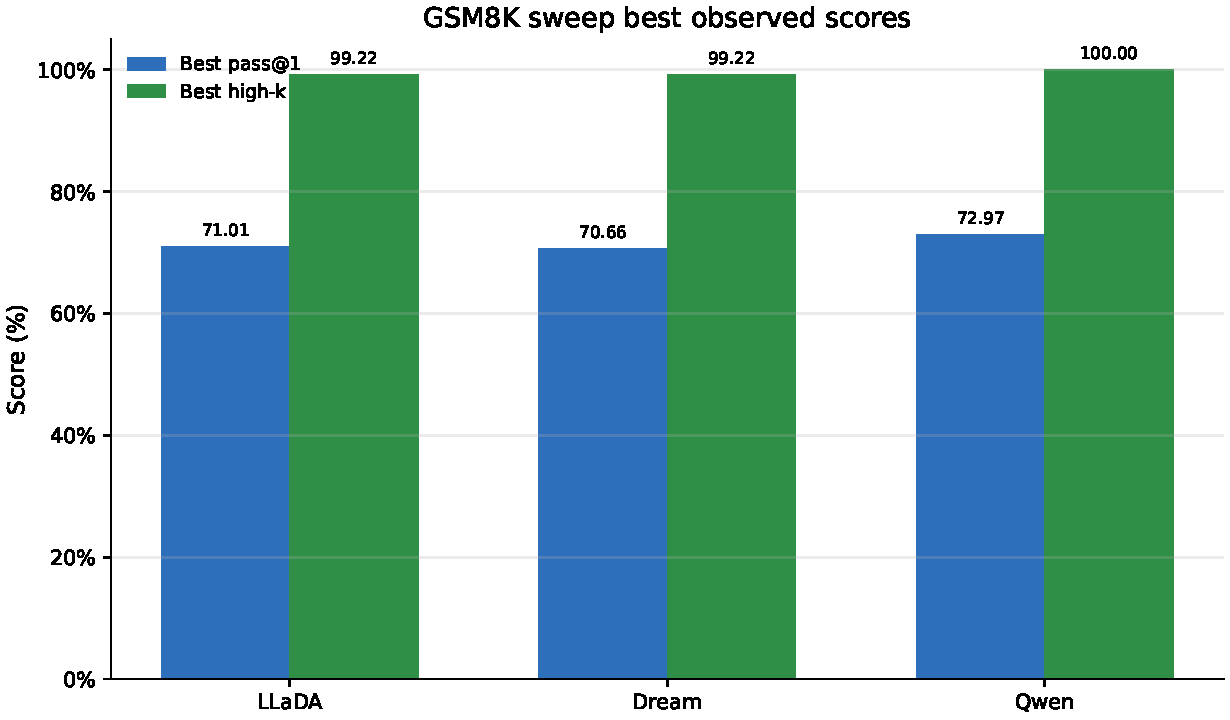
\includegraphics[width=0.78\textwidth]{images/hyperparameter_summary.pdf}
\caption{GSM8K sweep summary. The sweep motivates the controlled comparison by showing that tuning matters, but that the central pass@k ranking question remains after reasonable configurations are chosen.}
\label{fig:hyperparams}
\end{figure}

The sweep confirms that generation length is the dominant quality lever. Step count is decisive only for LLaDA, and Dream's effective step count is bounded below by the fast-dLLM scheduler regardless of the user-set parameter. Section~\ref{sec:results-countdown} therefore reports paradigm comparisons at fixed dataset-appropriate generation lengths and treats the diffusion-step parameter as a mostly latent backend choice.
